% Search for all the places that say "PUT SOMETHING HERE".

\documentclass[11pt]{article}
\usepackage{amsmath,textcomp,amssymb,graphicx,enumerate,hyperref,enumitem,mathtools,tikz-qtree,listings,chemformula,bm,graphicx,grffile,gensymb}
\graphicspath{{/Users/jonathansun5/Documents/Fall 2017/MCB 166/Homeworks/Screen Shot 2017-09-18 at 4.46.09 AM.png} {/Users/jonathansun5/Documents/Fall 2017/MCB 166/Homeworks/Screen Shot 2017-09-19 at 12.39.28 AM.png} {/Users/jonathansun5/Documents/Fall 2017/MCB 166/Homeworks/Screen Shot 2017-09-18 at 4.44.36 AM.png} {/Users/jonathansun5/Documents/Fall 2017/MCB 166/Homeworks/Screen Shot 2017-09-18 at 4.41.06 AM.png} {/Users/jonathansun5/Documents/Fall 2017/MCB 166/Homeworks/Screen Shot 2017-09-18 at 3.41.31 AM.png} {/Users/jonathansun5/Documents/Fall 2017/MCB 166/Homeworks/Screen Shot 2017-09-18 at 4.34.56 AM.png}}

\makeatletter
\newcommand{\leqnos}{\tagsleft@true\let\veqno\@@leqno}
\newcommand{\reqnos}{\tagsleft@false\let\veqno\@@eqno}
\reqnos
\makeatother

\def\Name{Jonathan Sun}  % Your name
\def\SID{25020651}  % Your student ID number
\def\Homework{1} % Number of Homework
\def\Session{Fall 2017}


\title{MCB166 --- \Session --- Problem Set \Homework}
\author{\Name, SID \SID}
\markboth{MCB166 --- \Session --- Problem Set \Homework --- \Name}{MCB166 --- \Session --- Problem Set \Homework --- \Name}
\pagestyle{myheadings}
\date{}

\def\endproofmark{$\Box$}
\newenvironment{proof}{\par{\bf Proof:}}{\endproofmark\smallskip}

\usepackage[margin=1in]{geometry}



\begin{document}
\maketitle

\newpage
\begin{enumerate}[label=\arabic*.]
\item
A \ch{Na}-selective ion channel that produces a single-channel current of $1.6$ pA (1 pA $= 10^{-12}$ amps) under a voltage of $90$ mV has a conductance of $17.8$ pS. Say that this channel is a membrane-spanning circular cylinder ($50$ Angstrom long) filled with a typical biological electrolyte soution (resistivity, $\rho = 60$ ohm-cm). Find the internal diameter of the pore. You will get a reasonable value for macromolecular pore, but would expect a Na-ion-selective pore to have a larger or smaller internal diameter? Draw a channel shape (not a uniform diameter cylinder) which can have the observed conductance as well as selectivity. (Hint: The molecular current picture of a channel profile would have a separate `vestibule' region and a `selectivity filter').
\begin{center}
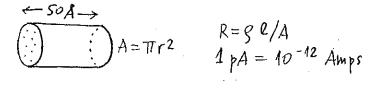
\includegraphics[width=0.5\textwidth]{/Users/jonathansun5/Documents/Fall 2017/MCB 166/Homeworks/Screen Shot 2017-09-18 at 4.46.09 AM.png}
\end{center}
To solve this problem, I will use the formula that $R = \frac{\rho \ell} {A}$:
\begin{align*}
R = \frac{\rho \ell} {A}
\end{align*}
\begin{align*}
R = \frac{\left(0.6\Omega \text{m}\right) \left(50 \times 10^{-10} \text{m}\right)} {\pi r^2}
\end{align*}
Because $R = \frac{1} {\sigma}$:
\begin{align*}
R = \frac{1} {17.8 \times 10^{-12} \text{S}} \approx 5.618 \times 10^{10} \Omega
\end{align*}
Therefore, we can set both equations equal to each other as:
\begin{align*}
5.618 \times 10^{10} \Omega \approx \frac{\left(0.6\Omega \text{m}\right) \left(50 \times 10^{-10} \text{m}\right)} {\pi r^2}
\end{align*}
\begin{align*}
r^2 \approx 1.69977 \times 10^{-20} \text{m}^2
\end{align*}
\begin{align*}
r \approx 1.30375 \times 10^{-10} \text{m}
\end{align*}
\begin{align*}
d = 2r \approx 2 \times 1.30375 \times 10^{-10} \text{m} \approx 2.60750 \times 10^{-10} \text{m}
\end{align*}
\vspace*{1\baselineskip}
\\
Therefore, we get that the internal diameter of the pore is approximately $2.60750 \times 10^{-10} \text{m}$.
\vspace*{1\baselineskip}
\\
To solve the second part of the problem, I will use the following diagram as an example:
\begin{center}
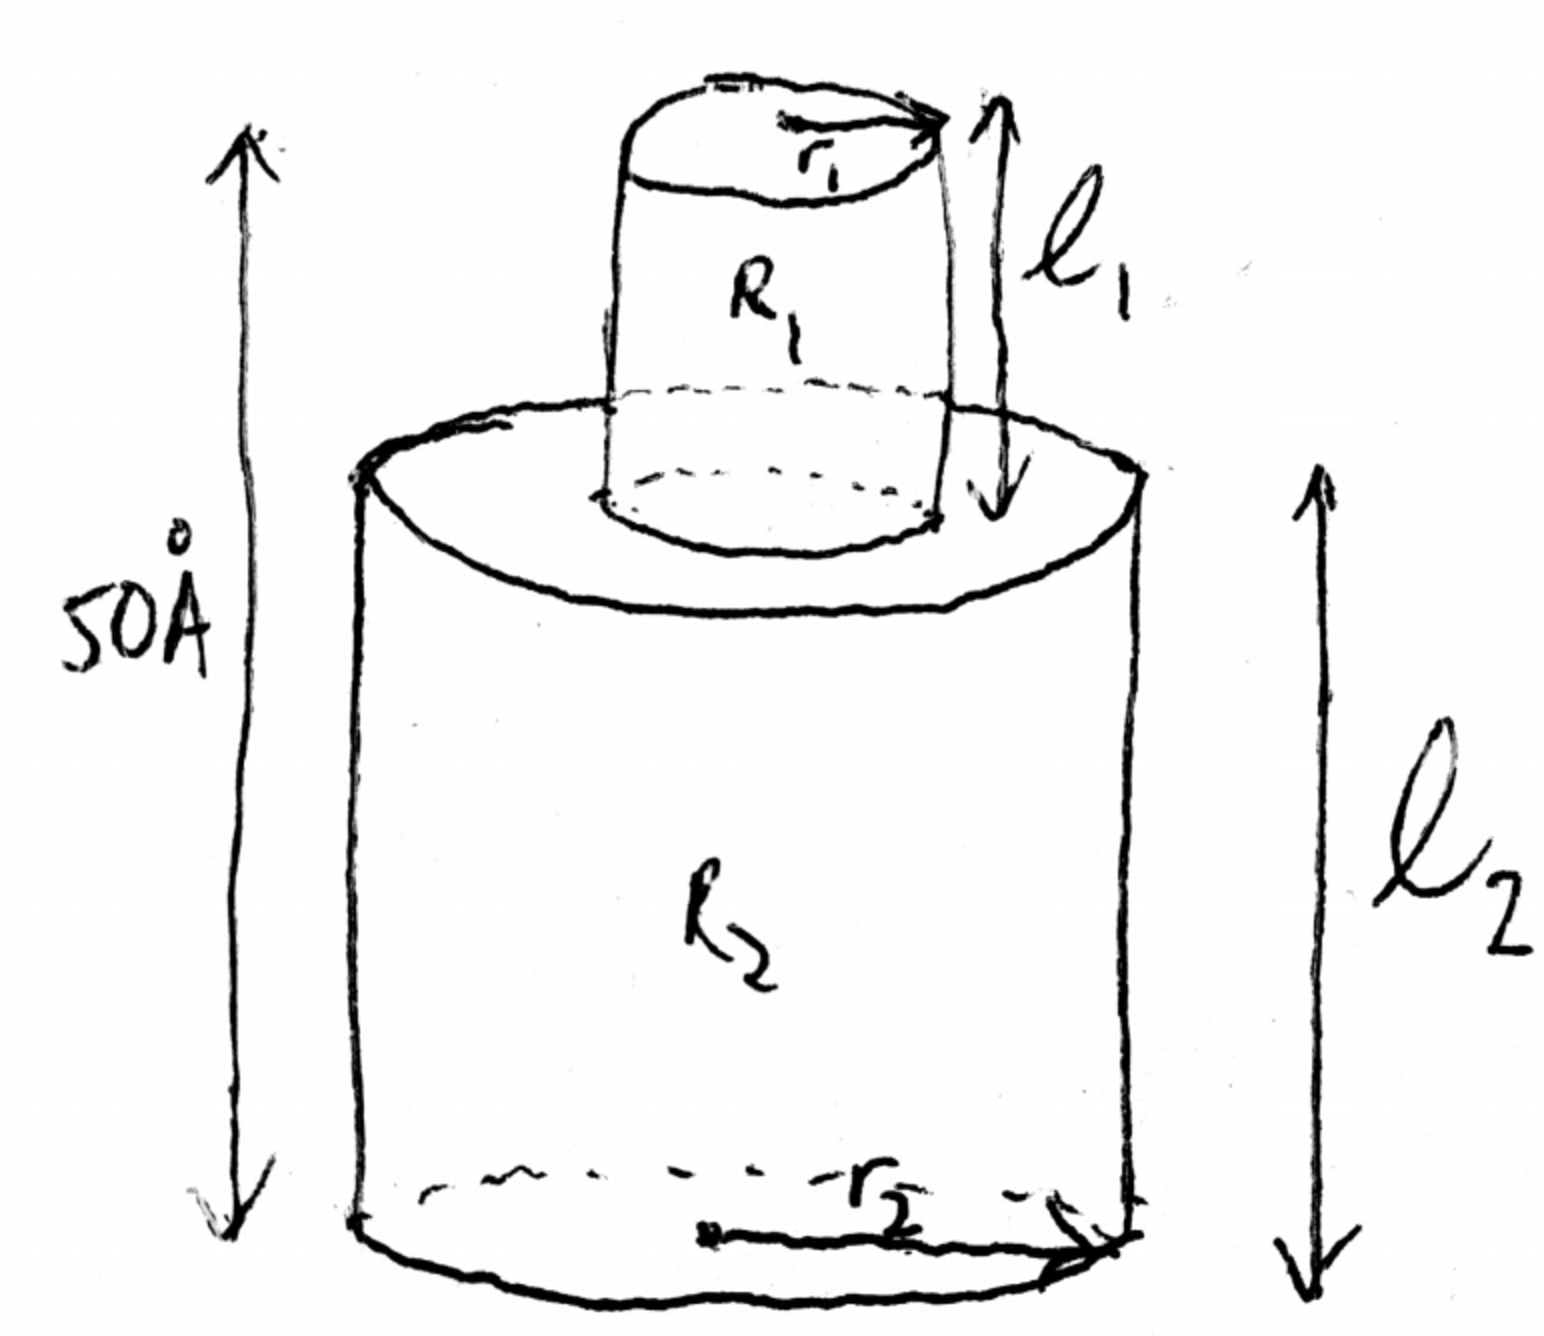
\includegraphics[width=0.5\textwidth]{/Users/jonathansun5/Documents/Fall 2017/MCB 166/Homeworks/Screen Shot 2017-09-19 at 12.39.28 AM.png}
\end{center}
This gives me the formula of:
\begin{align*}
R = R_1 + R_2
\end{align*}
\begin{align*}
R = \frac{\rho \ell_1} {A_1} + \frac{\rho \ell_2} {A_2}
\end{align*}
\begin{align*}
R = \frac{\rho \ell_1} {\pi r_1^2} + \frac{\rho \ell_2} {\pi r_2^2}
\end{align*}
Since $\ell_1 + \ell_2 = \ell$ we can rewrite the equation as:
\begin{align*}
R = \frac{\rho \left(\ell - \ell_2\right)} {\pi r_1^2} + \frac{\rho \ell_2} {\pi r_2^2}
\end{align*}
I will assume that $\ell_2 = 4r_2$ since it fits:
\begin{align*}
R = \frac{\rho \left(\ell - 4r_2\right)} {\pi r_1^2} + \frac{\rho \left(4r_2\right)} {\pi r_2^2}
\end{align*}
Since $R \approx 5.618 \times 10^{10} \Omega$, $\rho = 0.6 \Omega \text{m}$, and $\ell = 50 \text{A} = 50 \times 10^{-10} \text{m}$:
\begin{align*}
5.618 \times 10^{10} \Omega = \frac{0.6 \Omega \text{m} \left(50 \times 10^{-10} \text{m} - 4r_2\right)} {\pi r_1^2} + \frac{0.6 \Omega \text{m} \left(4r_2\right)} {\pi r_2^2}
\end{align*}
Passing in $r_1 \approx 1.30375 \times 10^{-10} \text{m}$:
\begin{align*}
5.618 \times 10^{10} \Omega = \frac{0.6 \Omega \text{m} \left((50 \times 10^{-10} \text{m}) - 4r_2\right)} {\pi (1.30375 \times 10^{-10} \text{m})^2} + \frac{0.6 \Omega \text{m} \left(4r_2\right)} {\pi r_2^2}
\end{align*}
\begin{align*}
r_2^2 \approx 1.69979 \text{m}^2
\end{align*}
\begin{align*}
r_2 \approx 1.30376 \times 10^{-10} \text{m}
\end{align*}
\begin{align*}
d_2 = 2r_2 \approx 2 \times 1.30376 \times 10^{-10} \text{m} \approx 2.60752 \times 10^{-10} \text{m}
\end{align*}
Since $d_2 \approx 2.60752 \times 10^{-10} \text{m}$ and this is basically equivalent to $d_1 \approx 2.60750 \times 10^{-10} \text{m}$, I would expect a \ch{Na}-ion-selective
pore to have approximately a same size internal diameter or one that is slightly larger.



\newpage
\item
The amplitude of a nerve action is about a $100$ mV displacement of the membrane potential caused by an influx of \ch{Na+} ions. How many moles of a monovalent ion must cross the membrane to set up a potential of this magnitude? ($C = 1$ microfarad per square centimeter of membrane). A squid giant axon has a diameter of $1$ mm, and the axoplasm has a ionic concentration of about $0.5$ M. Compare the number of ions needed to maintain a $100$ mV potential in $1$ cm$^2$ of membrane to the number in the axon cylinder enclosed by a $1$ cm$^2$ of membrane. A garfish olfactory nerve is $1$ micrometer in diameter ($10^{-3}$ mm). Do the same comparison for it. What does this calculation tell you about the running down of nerve batteries by the firing of action potentials?
\begin{center}
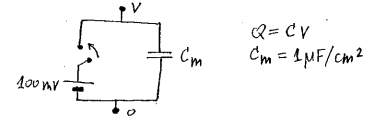
\includegraphics[width=0.5\textwidth]{/Users/jonathansun5/Documents/Fall 2017/MCB 166/Homeworks/Screen Shot 2017-09-18 at 4.44.36 AM.png}
\end{center}
To solve the first part of this problem, I will use $Q = C V$:
\begin{align*}
Q = C V
\end{align*}
Since $C = 1 \frac{\mu \text{F}} {\text{cm}^2}$ and $V = 100 \text{mV}$:
\begin{align*}
Q = \left(1 \frac{\mu \text{F}} {\text{cm}^2}\right) \left(100 \text{mV}\right)
\end{align*}
\begin{align*}
Q = \left(1 \frac{\mu \text{F}} {\text{cm}^2}\right) \left(\frac{10000 \text{cm}^2} {1 \text{m}^2}\right) \left(\frac{1\text{F}} {0.000001 \mu \text{F}}\right) \left(100 \text{mV}\right) \left(\frac{1\text{V}} {1000\text{mV}}\right)
\end{align*}
\begin{align*}
Q = 1000000000 \frac{\text{FV}} {\text{m}^2}
\end{align*}
Taking $\frac{Q} {e}$ where $e = \text{elementary electrical charge} = 1.602 \times 10^{-19} C$ will give me the number of ions per square meter:
\begin{align*}
\frac{Q} {e} = \frac{1000000000 \frac{\text{FV}} {\text{m}^2}} {1.602 \times 10^{-19} C}
\end{align*}
Since $C = \text{Coulomb} = \text{F} \times \text{V}$ we can rewrite the equation as:
\begin{align*}
\frac{Q} {e} = \frac{1000000000 \frac{\text{FV}} {\text{m}^2}} {1.602 \times 10^{-19} \text{FV}}
\end{align*}
\begin{align*}
\frac{Q} {e} = \frac{1000000000 \frac{\text{FV}} {\text{m}^2}} {1.602 \times 10^{-19} \text{FV}}
\end{align*}
\begin{align*}
\frac{Q} {e} \approx 6.242197 \times 10^{27} \frac{\text{molecules}} {\text{m}^2}
\end{align*}
Taking the answer from above and dividing it with Avagadro's Number gives us:
\begin{align*}
\frac{6.242197 \times 10^{27} \frac{\text{molecules}} {\text{m}^2}} {N_A} \approx \frac{6.242197 \times 10^{27} \frac{\text{molecules}} {\text{m}^2}} {6.023 \times 10^{23} \frac{\text{molecules}} {\text{mole}}} \approx 10363.933 \frac{\text{mole}} {\text{m}^2} = 1.0363933 \frac{\text{mole}} {\text{cm}^2} \approx 1 \frac{\text{mole}} {\text{cm}^2}
\end{align*}
Therefore, approximately $10363.933$ moles of a monovalent ion per square meter or $1$ mole of a monovalent ion per square centimeter must cross the membrane to set up a potential of this magnitude.
\vspace*{1\baselineskip}
\\
To solve the next part of the problem, I will first solve for the volume while using the surface area of the squid axon:
\begin{align*}
d = 1 \text{mm}
\end{align*}
\begin{align*}
r = 0.5 \text{mm} = 5 \times 10^{-4} \text{m}
\end{align*}
\begin{align*}
\text{SA} = 2 \pi r \ell
\end{align*}
\begin{align*}
\text{V} = \pi r^2 \ell
\end{align*}
\begin{align*}
\text{V} = \frac{\text{SA} \times r} {2}
\end{align*}
\begin{align*}
\text{V} = \frac{\text{SA} \times r} {2}
\end{align*}
Since we are working with $1 \text{cm}^2 = 10^{-4} \text{m}^2$ of the membrane:
\begin{align*}
\text{V} = \frac{10^{-4} \text{m}^2 \times 5 \times 10^{-4} \text{m}} {2}
\end{align*}
\begin{align*}
\text{V} = 2.5 \times 10^{-8} \text{m}^3
\end{align*}
Since the ionic concentration of about $0.5 \text{M}$ and I need to convert volume to liters:
\begin{align*}
2.5 \times 10^{-8} \text{m}^3 = 2.5 \times 10^{-5} \text{L}
\end{align*}
\begin{align*}
0.5 \frac{\text{mol}} {L} \times 2.5 \times 10^{-5} \text{L} = 1.25 \times 10^{-5} \text{mol}
\end{align*}
Therefore, we get $1.25 \times 10^{-5} \text{mol}$ for the squid axon.
\vspace*{1\baselineskip}
\\
To solve the next part of the problem, I will do the same thing above except work with a $1 \text{micrometer}$ diameter:
\begin{align*}
d = 1 \mu \text{m}
\end{align*}
\begin{align*}
r = 0.5 \mu \text{m} = 0.5 \times 10^{-6} \text{m}
\end{align*}
\begin{align*}
\text{V} = \frac{\text{SA} \times r} {2}
\end{align*}
\begin{align*}
\text{V} = \frac{10^{-4} \text{m}^2 \times 0.5 \times 10^{-6} \text{m}} {2}
\end{align*}
\begin{align*}
\text{V} = \frac{0.5 \times 10^{-10} \text{m}^3} {2} = 0.25 \times 10^{-10} \text{m}^3 = 2.5 \times 10^{-11} \text{m}^3
\end{align*}
Again, since the ionic concentration of about $0.5 \text{M}$ and I need to convert volume to liters:
\begin{align*}
2.5 \times 10^{-11} \text{m}^3 = 2.5 \times 10^{-8} \text{L}
\end{align*}
\begin{align*}
0.5 \frac{\text{mol}} {L} \times 2.5 \times 10^{-8} \text{L} = 1.25 \times 10^{-8} \text{mol}
\end{align*}
Therefore, we get $1.25 \times 10^{-8} \text{mol}$ for the garfish olfactory nerve.



\newpage
\item
Consider the membrane equivalent circuit shown in class. Instead of constant-current generator, the cell is now stimulated by a battery of potential V$_c$ via a high-resistance microelectrode, $R_e = 1 / g_e$. (For a typical glass microelectrode, $R_e = 10^7$ ohm).
\begin{center}
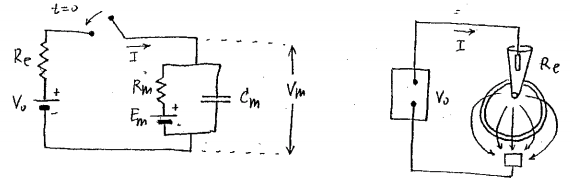
\includegraphics[width=1\textwidth]{/Users/jonathansun5/Documents/Fall 2017/MCB 166/Homeworks/Screen Shot 2017-09-18 at 4.41.06 AM.png}
\end{center}
\begin{enumerate}[label=(\alph*)]
\item
Write the differential equation for the membrane potential as a function of time after V$_c$ is instantaneously switched on.
\vspace*{1\baselineskip}
\\
That is, apply Kirchoff's laws to the circuit having parallel leak and capacitance currents. Because of the large resistance of the microelectrode, the applied pulse will be characterized by two time constants, the membrane time constant, $T_m = R_mC_m = 10^{-3}$ sec independent of the size of the cell, and an additional `access-resistance' time constant, $T_e = R_eC_m$, which will depend on the size of the cell (for a cell of area $100$ square microns, $C_m = 10^{-6}$farads/cm$^2$ x $100$ x $10^{-8}$cm$^2 = 10^{-12}$ farads; hence for this particular cell, $T_e = 10^7$ ohms x $10^{-12}$ farads $= 10^{-5}$ sec). This means when an experimenter applies a fast step of voltage to the electrode the membrane potential V$_m$ cannot follow instantaneously and dows not reach a value equal to the applied potential.
\vspace*{1\baselineskip}
\\
In fact, I'll even give you the answer, but you must show the steps to get there. \\
\begin{equation}
\label{eq:1}
dV_m / dt + V_m / T = V_o / T_e + E_m / T_m
\end{equation}
\begin{align*}
\text{where} && T_e = R_eC_m = C_m / g_e \text{,} && T_m = R_mC_m = C_m / g_m \text{,} && 1/T = 1/T_e + 1/T_m
\end{align*}
\vspace*{1\baselineskip}
\\
To get to equation $(1)$, I will need to Kirchoff's current law:
\begin{align*}
I_{total} = I_{capacitive} + I_{resistive}
\end{align*}
I will break this equation into $3$ parts: $I_{total}$, $I_{capacitive}$, and $I_{resistive}$. \\

\boldsymbol{$I_{total}:$}
\begin{align*}
V_e = I_{total} R_e
\end{align*}
\begin{align*}
V_o = V_e + V_m
\end{align*}
Substituting the second equation into the first one we get:
\begin{align*}
I_{total} = \frac{V_o - V_m} {R_e}
\end{align*}

\boldsymbol{$I_{capacitive}:$}
\begin{align*}
I_c = \frac{dQ} {dt}
\end{align*}
\begin{align*}
Q = C_m\Delta V_m
\end{align*}
Taking the derivative in respect to time we get:
\begin{align*}
\frac{dQ} {dt} = C_m \frac{dV_m} {dt}
\end{align*}
\begin{align*}
I_c = C_m \frac{dV_m} {dt}
\end{align*}

\boldsymbol{$I_{resistive}:$}
\begin{align*}
V_m = E_m + I_r R_m
\end{align*}
\begin{align*}
I_r = \frac{V_m - E_m} {R_m}
\end{align*}

Therefore, $I_{total} = I_{capacitive} + I_{resistive}$ is equivalent to:
\begin{align*}
\frac{V_o - V_m} {R_e} = C_m \frac{dV_m} {dt} + \frac{V_m - E_m} {R_m}
\end{align*}
By rearranging the equation we get:
\begin{align*}
\frac{V_o - V_m} {R_e} - \frac{V_m - E_m} {R_m} = C_m \frac{dV_m} {dt}
\end{align*}
We are given that $T_e = R_e C_m$ and $T_m = R_m C_m$ which means $C_m = \frac{T_m} {R_m}$, $R_m = \frac{T_m} {C_m}$, and $R_e = \frac{T_e} {C_m}$. We can rewrite the equation above as:
\begin{align*}
\frac{V_o} {R_e} - \frac{V_m} {R_e} - \frac{V_m} {R_m} + \frac{E_m} {R_m} = \frac{T_m} {R_m} \frac{dV_m} {dt}
\end{align*}
\begin{align*}
 \frac{R_m} {T_m} (\frac{V_o} {R_e} - \frac{V_m} {R_e} - \frac{V_m} {R_m} + \frac{E_m} {R_m}) = \frac{dV_m} {dt}
\end{align*}
\begin{align*}
\frac{R_m V_o} {R_e T_m} - \frac{R_m V_m} {R_e T_m} - \frac{V_m} {T_m} + \frac{E_m} {T_m} = \frac{dV_m} {dt}
\end{align*}
\begin{align*}
\frac{T_m V_o} {T_e T_m} - \frac{T_m V_m} {T_e T_m} - \frac{V_m} {T_m} + \frac{E_m} {T_m} = \frac{dV_m} {dt}
\end{align*}
\begin{align*}
\frac{V_o} {T_e} - \frac{V_m} {T_e} - \frac{V_m} {T_m} + \frac{E_m} {T_m} = \frac{dV_m} {dt}
\end{align*}
\begin{align*}
\frac{V_o - V_m} {T_e} - \frac{V_m} {T_m} + \frac{E_m} {T_m} = \frac{dV_m} {dt}
\end{align*}
Since $\frac{1} {T} = \frac{1} {T_e} + \frac{1} {T_m}$ this means that $\frac{1} {T_e} = \frac{1} {T} - \frac{1} {T_m}$. We can rewrite the equation above as:
\begin{align*}
\left(V_o - V_m\right)\left(\frac{1} {T} - \frac{1} {T_m}\right) - \frac{V_m} {T_m} + \frac{E_m} {T_m} = \frac{dV_m} {dt}
\end{align*}
\begin{align*}
\frac{V_o} {T} - \frac{V_o} {T_m} - \frac{V_m} {T} + \frac{V_m} {T_m} - \frac{V_m} {T_m} + \frac{E_m} {T_m} = \frac{dV_m} {dt}
\end{align*}
\begin{align*}
\frac{V_o} {T} - \frac{V_o} {T_m} - \frac{V_m} {T} + \frac{E_m} {T_m} = \frac{dV_m} {dt}
\end{align*}
\begin{align*}
\frac{V_o} {T} - \frac{V_o} {T_m} + \frac{E_m} {T_m} = \frac{dV_m} {dt} + \frac{V_m} {T}
\end{align*}
\begin{align*}
V_o\left(\frac{1} {T_e} + \frac{1} {T_m}\right) - \frac{V_o} {T_m} + \frac{E_m} {T_m} = \frac{dV_m} {dt} + \frac{V_m} {T}
\end{align*}
\begin{align*}
\frac{V_o} {T_e} + \frac{V_o} {T_m} - \frac{V_o} {T_m} + \frac{E_m} {T_m} = \frac{dV_m} {dt} + \frac{V_m} {T}
\end{align*}
\begin{align*}
\frac{V_o} {T_e} + \frac{E_m} {T_m} = \frac{dV_m} {dt} + \frac{V_m} {T}
\end{align*}
Since the equation is equivalent to $\frac{dV_m} {dt} + \frac{V_m} {T} = \frac{V_o} {T_e} + \frac{E_m} {T_m}$, we have solved this problem.



\newpage
\item
Verify that Eqn (2) below is the solution to Eqn(1) satisfying the initial condition that $\text{V}_\text{m} = \text{E}_\text{m}$ until the switch is thrown. \\
\begin{equation}
\label{eq:2}
V_m(t) = [(R_m V_o + R_e E_m) / (R_m + R_e)] (1 - \text{exp}(-t / T)) + E_m \text{exp}(-t / T) \\
\end{equation}
\begin{align*}
\text{or} && V_m(t) - E_m = (R_m / (R_e+ R_m)) (V_o - E_m) (1 - \text{exp}(-t / T))
\end{align*}
To verify that Eqn (2) is the solution to Eqn(1) regards to $\text{V}_\text{m} = \text{E}_\text{m}$ until the switch is thrown means that we can use $t = 0$ since the equations need to match at $t = 0$.
\vspace*{1\baselineskip}
\\
For Eqn(1):
\begin{equation}
\tag{\ref{eq:1}}
\frac{dV_m} {dt} + \frac{V_m} {T} = \frac{V_o} {T_e} + \frac{E_m} {T_m}
\end{equation}
\begin{align*}
V_m(t) = e^{\frac{-t} {T}} \left(\frac{V_o} {T_e} + \frac{E_m} {T_m}\right) \int e^{\frac{t} {T}}\mathrm{d}t
\end{align*}
\begin{align*}
V_m(t) = e^{\frac{-t} {T}} \left(\frac{V_o} {T_e} + \frac{E_m} {T_m}\right)\left(Te^{\frac{t} {T}} + C\right)
\end{align*}
Since $t = 0$ and $V_m(0) = E(m)$ we can rewrite the equation above and solve for $C$:
\begin{align*}
E_m = e^{\frac{0} {T}} \left(\frac{V_o} {T_e} + \frac{E_m} {T_m}\right)\left(Te^{\frac{0} {T}} + C\right)
\end{align*}
\begin{align*}
E_m = \left(\frac{V_o} {T_e} + \frac{E_m} {T_m}\right)\left(T + C\right)
\end{align*}
\begin{align*}
\frac{E_m} {\frac{V_o} {T_e} + \frac{E_m} {T_m}} = T + C
\end{align*}
\begin{align*}
\frac{E_m} {\frac{V_o T_m + E_m T_e} {T_e T_m}} = T + C
\end{align*}
\begin{align*}
\frac{E_m T_e T_m} {V_o T_m + E_m T_e} = T + C
\end{align*}
\begin{align*}
C = \frac{E_m T_e T_m} {V_o T_m + E_m T_e} - T
\end{align*}
Plugging $C$ back into our equation gives us:
\begin{align*}
V_m(t) = e^{\frac{-t} {T}} \left(\frac{V_o} {T_e} + \frac{E_m} {T_m}\right)\left(Te^{\frac{t} {T}} + \frac{E_m T_e T_m} {V_o T_m + E_m T_e} - T\right)
\end{align*}
Again, since $t = 0$ we can rewrite the equation above as:
\begin{align*}
V_m(0) = e^{\frac{0} {T}} \left(\frac{V_o} {T_e} + \frac{E_m} {T_m}\right)\left(Te^{\frac{0} {T}} + \frac{E_m T_e T_m} {V_o T_m + E_m T_e} - T\right)
\end{align*}
\begin{align*}
V_m(0) = \left(\frac{V_o} {T_e} + \frac{E_m} {T_m}\right)\left(T + \frac{E_m T_e T_m} {V_o T_m + E_m T_e} - T\right)
\end{align*}
\begin{align*}
V_m(0) = \left(\frac{V_o} {T_e} + \frac{E_m} {T_m}\right)\left(\frac{E_m T_e T_m} {V_o T_m + E_m T_e}\right)
\end{align*}
\begin{align*}
V_m(0) = \left(\frac{V_o T_m + E_m T_e} {T_e T_m}\right)\left(\frac{E_m T_e T_m} {V_o T_m + E_m T_e}\right)
\end{align*}
\begin{align*}
V_m(0) = E_m
\end{align*}
Thus, we got $V_m(0) = E_m$ for Eq(1).
\vspace*{1\baselineskip}
\\
For Eq(2) we nust also reach the same conclusion to solve this problem:
\begin{equation}
\tag{\ref{eq:2}}
V_m(t) = \left(\frac{R_m V_o + R_e E_m} {R_m + R_e}\right) \left(1 - e^{\frac{-t} {T}}\right) + E_m e^{\frac{-t} {T}}
\end{equation}
Since $t = 0$ we can rewrite the equation above as:
\begin{align*}
V_m(0) = \left(\frac{R_m V_o + R_e E_m} {R_m + R_e}\right) \left(1 - e^{\frac{0} {T}}\right) + E_m e^{\frac{0} {T}}
\end{align*}
\begin{align*}
V_m(0) = \left(\frac{R_m V_o + R_e E_m} {R_m + R_e}\right) \left(1 - 1\right) + E_m
\end{align*}
\begin{align*}
V_m(0) = \left(\frac{R_m V_o + R_e E_m} {R_m + R_e}\right) \left(0\right) + E_m
\end{align*}
\begin{align*}
V_m(0) = E_m
\end{align*}
Thus, we got $V_m(0) = E_m$ for Eq(2).
\vspace*{1\baselineskip}
\\
Since both Eqn(1) and Eqn(2) both arrived at the same conclusion that $V_m(0) = E_m$ when $t = 0$, we have shown that Eqn (2) is the solution to Eqn(1) regards to $\text{V}_\text{m} = \text{E}_\text{m}$ until the switch is thrown.



\newpage
\item
For our cell at rest, R$_m = 10^3$ ohm-cm$^2 / 10^{-6}$ cm$^2 = 10^9$ ohm. Find V$_m(\infty)$ compared to V$_o$. Say during excitation, the membrane resistances drops by a factor of $100$. What happens to V$_m(\infty)$ for a fixed V$_o$? Is our battery still a constant-voltage source in this case?
\vspace*{1\baselineskip}
\\
We start with Eqn(2):
\begin{align*}
V_m(t) - E_m = \left(\frac{R_m} {R_e+ R_m}\right) \left(V_o - E_m\right) \left(1 - e^{\frac{-t} {T}}\right)
\end{align*}
\begin{align*}
V_m(t) = E_m + \left(\frac{R_m} {R_e+ R_m}\right) \left(V_o - E_m\right) \left(1 - e^{\frac{-t} {T}}\right)
\end{align*}
\begin{align*}
V_m(\infty) = E_m + \left(\frac{R_m} {R_e+ R_m}\right) \left(V_o - E_m\right) \left(1 - e^{\frac{-\infty} {T}}\right)
\end{align*}
\begin{align*}
V_m(\infty) = E_m + \left(\frac{R_m} {R_e+ R_m}\right) \left(V_o - E_m\right) \left(1 - 0\right)
\end{align*}
\begin{align*}
V_m(\infty) = E_m + \left(\frac{R_m} {R_e+ R_m}\right) \left(V_o - E_m\right)
\end{align*}
Since $\text{R}_\text{m} = 10^9 \text{ohm}$ and $\text{R}_\text{e} = 10^7 \text{ohm}$:
\begin{align*}
V_m(\infty) = E_m + \left(\frac{10^9} {10^7 + 10^9}\right) \left(V_o - E_m\right)
\end{align*}
\begin{align*}
V_m(\infty) = E_m + \left(\frac{100} {101}\right) \left(V_o - E_m\right)
\end{align*}
\begin{align*}
V_m(\infty) = E_m + \frac{100} {101} V_o - \frac{100} {101} E_m
\end{align*}
\begin{align*}
V_m(\infty) = \frac{1} {101} E_m + \frac{100} {101} V_o
\end{align*}
\begin{align*}
V_m(\infty) \approx V_o
\end{align*}
Therefore, $V_m(\infty) \approx V_o$.
\vspace*{1\baselineskip}
\\
During excitation, since the membrane resistances drops by a factor of $100$ we need to change $\text{R}_\text{m} = 10^9 \text{ohm}$ to $\text{R}_\text{m} = 10^7 \text{ohm}$:
\begin{align*}
V_m(\infty) = E_m + \left(\frac{R_m} {R_e+ R_m}\right) \left(V_o - E_m\right)
\end{align*}
\begin{align*}
V_m(\infty) = E_m + \left(\frac{10^7} {10^7 + 10^7}\right) \left(V_o - E_m\right)
\end{align*}
\begin{align*}
V_m(\infty) = E_m + \left(\frac{1} {2}\right) \left(V_o - E_m\right)
\end{align*}
\begin{align*}
V_m(\infty) = E_m + \frac{1} {2} V_o - \frac{1} {2} E_m
\end{align*}
\begin{align*}
V_m(\infty) = \frac{1} {2} E_m + \frac{1} {2} V_o
\end{align*}
Therefore, $V_m(\infty) = \frac{1} {2} E_m + \frac{1} {2} V_o$ when the cell is excited.
\vspace*{1\baselineskip}
\\
Because $\text{V}_\text{m}(\infty)$ when the cell is at rest and when the cell is excited are not equivalent $\left(V_o \neq \frac{1} {2} E_m + \frac{1} {2} V_o\right)$, our battery still not a constant-voltage source.



\end{enumerate}





\newpage
\item
The figure shows data for a cell with \ch{Na+} and \ch{K+} as the only permeable ions. For this case, the Goldman equation can be written as \\
\begin{align*}
Vm && = && (kT/e) \ln{[(P_{\ch{K}}[\ch{K+}]_o + P_{\ch{Na}}[\ch{Na+}]_o) / (P_{\ch{K}}[\ch{K+}]_i + P_{\ch{Na}}[\ch{Na+}]_i)]} \\
&& = && 60\log_{10}{[([\ch{K+}]_o + r[\ch{Na+}]_o) / ([\ch{K+}]_i + r[\ch{Na+}]_i)]}
\end{align*}
where $r = P_{\ch{Na}} / P_{\ch{K}}$ is the relative permeability. For this cell, the external \ch{Na} is held fixed at $50$ mM. Find $r$ from the data given. (Hint: one way to solve this provlem is to notice that the dashed line represents data for which the \ch{Na+} contribution is negligible since it has the slope appropriate to perfect \ch{K+} selectivity. The horizontal line is asymptotic to the condition $[\ch{K}]_o = 0$. The two lines intersect $\log_{10}([\ch{K}]_o)$ or $[\ch{K}]_o = 5$ mM).
\begin{center}
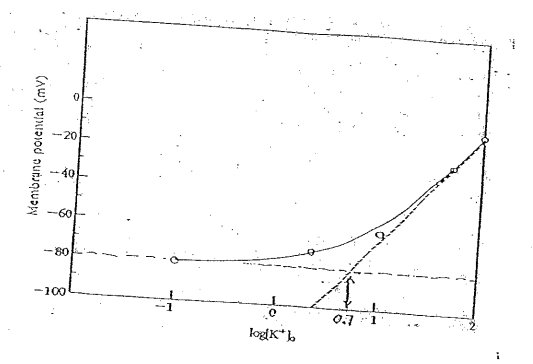
\includegraphics[width=1\textwidth]{/Users/jonathansun5/Documents/Fall 2017/MCB 166/Homeworks/Screen Shot 2017-09-18 at 3.41.31 AM.png}
\end{center}
To solve this problem, I will consider when $\log_{10}{[\ch{K+}]_o} \to -\infty$ and $\log_{10}{[\ch{K+}]_o} \to \infty$.
\vspace*{1\baselineskip}
\\
\boldsymbol{${\log_{10}{[\ch{K+}]_o}} \to -\infty:$} \\
As $\log_{10}{[\ch{K+}]_o} \to -\infty$, $[\ch{K+}]_o \to 0$.
\begin{align*}
V_m = 60\log_{10}{\frac{[\ch{K+}]_o + r[\ch{Na+}]_o} {[\ch{K+}]_i + r[\ch{Na+}]_i}}
\end{align*}
\begin{align*}
V_m = 60\log_{10}{\frac{r[\ch{Na+}]_o} {[\ch{K+}]_i + r[\ch{Na+}]_i}}
\end{align*}
\begin{align*}
V_m = 60\log_{10}{(r[\ch{Na+}]_o)} - 60\log_{10}{([\ch{K+}]_i + r[\ch{Na+}]_i)}
\end{align*}

\boldsymbol{${\log_{10}{[\ch{K+}]_o}} \to \infty:$} \\
As $\log_{10}{[\ch{K+}]_o} \to \infty$, $r[\ch{Na+}]_o$ becomes so insignificant so I can leave it out.
\begin{align*}
V_m = 60\log_{10}{\frac{[\ch{K+}]_o + r[\ch{Na+}]_o} {[\ch{K+}]_i + r[\ch{Na+}]_i}}
\end{align*}
\begin{align*}
V_m = 60\log_{10}{\frac{[\ch{K+}]_o} {[\ch{K+}]_i + r[\ch{Na+}]_i}}
\end{align*}
\begin{align*}
V_m = 60\log_{10}{([\ch{K+}]_o)} - 60\log_{10}{([\ch{K+}]_i + r[\ch{Na+}]_i)}
\end{align*}
Since the two lines intersect at $\log_{10}([\ch{K+}]o) \approx 0.7$, we will plug this into the equation above.
\begin{align*}
-80 = 60(0.7) - 60\log_{10}{([\ch{K+}]_i + r[\ch{Na+}]_i)}
\end{align*}
\begin{align*}
-80 = 42 - 60\log_{10}{([\ch{K+}]_i + r[\ch{Na+}]_i)}
\end{align*}
\begin{align*}
-122 = - 60\log_{10}{([\ch{K+}]_i + r[\ch{Na+}]_i)}
\end{align*}
Plugging this into $V_m = 60\log_{10}{(r[\ch{Na+}]_o)} - 60\log_{10}{([\ch{K+}]_i + r[\ch{Na+}]_i)}$ we get:
\begin{align*}
-80 = 60\log_{10}{(r[\ch{Na+}]_o)} - 122
\end{align*}
\begin{align*}
42 = 60\log_{10}{(r[\ch{Na+}]_o)}
\end{align*}
\begin{align*}
0.7 = \log_{10}{(r[\ch{Na+}]_o)}
\end{align*}
\begin{align*}
10^{0.7} = 10^{\log_{10}{(r[\ch{Na+}]_o)}}
\end{align*}
\begin{align*}
10^{0.7} = r[\ch{Na+}]_o
\end{align*}
Since the question states that $[\ch{Na+}]_o = 50mM$, we can plug this in to solve for $r$:
\begin{align*}
10^{0.7} = 50r
\end{align*}
\begin{align*}
r \approx 0.100237
\end{align*}
Therefore, the relative permeability is about $0.100237$.



\newpage
\item
The membrane situation shown is a Donnan equilibrium. The external permeant ion concentrations given as $[\ch{K+}]_o = 10$ mM and $[\ch{Cl-}]_o = 200$ mM and impermeant $[\ch{Na+}]_o = 190$ mM. The internal impermeant (monovalent) anion concentration is $[\ch{A-}] = 100$ mM. Find the concentrations $[\ch{K+}]_i$ and $[\ch{Cl-}]_i$ and find the Donnan equilibrium potential across the membrane. Recall that the internal and external solutions are electroneutral; there is osmotic equilibrium; and the permeant ions must be at equilibrium at the same membrane potential (Donnan condition).
\begin{center}
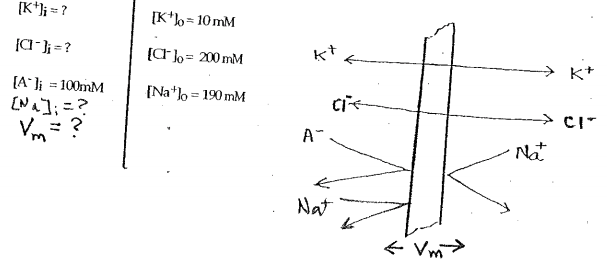
\includegraphics[width=1\textwidth]{/Users/jonathansun5/Documents/Fall 2017/MCB 166/Homeworks/Screen Shot 2017-09-18 at 4.34.56 AM.png}
\end{center}
\begin{align*}
\text{Osmotic Equilibrium:} && [\ch{K+}]_i + [\ch{Na+}]_i + [\ch{A-}]_i + [\ch{Cl-}]_i = [\ch{K+}]_o + [\ch{Na+}]_o + [\ch{Cl-}]_o
\end{align*}
\begin{align*}
\text{Electroneutrality:} && [\ch{K+}]_i + [\ch{Na+}]_i = [\ch{A-}]_i + [\ch{Cl-}]_i \\
&& [\ch{K+}]_o + [\ch{Na+}]_o = [\ch{Cl-}]_o
\end{align*}
\begin{align*}
\text{Donnan Equilibrium:} &&  \frac{\ch{K}_o} {\ch{K}_i} = \frac{\ch{Cl}_i} {\ch{Cl}_o}
\end{align*}

Using the Osmotic Equilibrium equation, we get:
\begin{align*}
[\ch{K+}]_i + [\ch{Na+}]_i + [\ch{A-}]_i + [\ch{Cl-}]_i = [\ch{K+}]_o + [\ch{Na+}]_o + [\ch{Cl-}]_o
\end{align*}
\begin{align*}
[\ch{K+}]_i + [\ch{Na+}]_i + 100 \text{ mM} + [\ch{Cl-}]_i = 10 \text{ mM} + 190 \text{ mM} + 200 \text{ mM}
\end{align*}
\begin{align*}
[\ch{K+}]_i + [\ch{Na+}]_i + [\ch{Cl-}]_i = 300 \text{ mM}
\end{align*}

Using the Electroneutrality equation, we get:
\begin{align*}
[\ch{K+}]_i + [\ch{Na+}]_i = [\ch{A-}]_i + [\ch{Cl-}]_i
\end{align*}
\begin{align*}
[\ch{K+}]_i + [\ch{Na+}]_i = 100 \text{ mM} + [\ch{Cl-}]_i
\end{align*}
\begin{align*}
[\ch{K+}]_i + [\ch{Na+}]_i - [\ch{Cl-}]_i= 100 \text{ mM}
\end{align*}

Using the Donnan Equilibrium equation, we get:
\begin{align*}
\frac{[\ch{K+}]_o} {[\ch{K+}]_i} = \frac{[\ch{Cl-}]_i} {[\ch{Cl-}]_o}
\end{align*}
\begin{align*}
\frac{10 \text{ mM}} {[\ch{K+}]_i} = \frac{[\ch{Cl-}]_i} {200 \text{ mM}}
\end{align*}
\begin{align*}
[\ch{Cl-}]_i [\ch{K+}]_i = 2000 \text{ mM}^2
\end{align*}

Subtracting the what we got from the Electroneutrality equation from what we got from the Osmotic Equilibrium equation, we get:
\begin{align*}
\begin{tabular}{cc}
  & $[\ch{K+}]_i + [\ch{Na+}]_i + [\ch{Cl-}]_i = 300 \text{ mM}$ \\
- & $[\ch{K+}]_i + [\ch{Na+}]_i - [\ch{Cl-}]_i= 100 \text{ mM}$ \\
\hline
  & $2[\ch{Cl-}]_i = 200 \text{ mM}$ \\
\end{tabular}
\end{align*}

This gives me:
\begin{align*}
[\ch{Cl-}]_i = 100 \text{ mM}
\end{align*}

Plugging in ($[\ch{Cl-}]_i = 100 \text{ mM}$) into what we got from the Donnan Equilibrium equation, we get:
\begin{align*}
[\ch{Cl-}]_i [\ch{K+}]_i = 2000 \text{ mM}^2
\end{align*}
\begin{align*}
(100 \text{ mM}) [\ch{K+}]_i = 2000 \text{ mM}^2
\end{align*}
\begin{align*}
[\ch{K+}]_i = 20 \text{ mM}
\end{align*}

Plugging in ($[\ch{Cl-}]_i = 100 \text{ mM}$) and ($[\ch{K+}]_i = 20 \text{ mM}$) into what we got from the Electroneutrality equation, we get:
\begin{align*}
[\ch{K+}]_i + [\ch{Na+}]_i - [\ch{Cl-}]_i= 100 \text{ mM}
\end{align*}
\begin{align*}
20 \text{ mM} + [\ch{Na+}]_i - 100 \text{ mM}= 100 \text{ mM}
\end{align*}
\begin{align*}
[\ch{Na+}]_i= 180 \text{ mM}
\end{align*}

To find the Donnan equilibrium potential across the membrane, we will use:
\begin{align*}
E_{m, \ch{K}} = \frac{RT} {F} \ln{\left(\frac{[\ch{K+}]_o} {[\ch{K+}]_i}\right)}
\end{align*}
\begin{align*}
E_{m, \ch{Na}} = \frac{RT} {F} \ln{\left(\frac{[\ch{Na+}]_o} {[\ch{Na+}]_i}\right)}
\end{align*}
\begin{align*}
E_{m, \ch{Cl}} = \frac{RT} {F} \ln{\left(\frac{[\ch{Cl-}]_i} {[\ch{Cl-}]_o}\right)}
\end{align*}
Assuming that $T = 25\text{\degree C} = 298.15 \text{K}$ and using $R = \text{gas constant} = 1.987 \frac{\text{cal}}{\text{K} \times \text{mol}} = 1.987 \times 10^{-3} \frac{\text{kcal}}{\text{K} \times \text{mol}} = 8.314 \frac{\text{C} \times \text{V}} {\text{K} \times \text{mol}}$ and $F = \text{Faraday's constant} = 9.648 \times 10^4 \frac{\text{C}} {\text{mol}}$ we can solve for the Donnan equilibrium potential across the membrane for each element:
\begin{align*}
E_{m, \ch{K}} = \frac{RT} {F} \ln{\left(\frac{[\ch{K+}]_o} {[\ch{K+}]_i}\right)} = \frac{{8.314 \frac{\text{C} \times \text{V}} {\text{K} \times \text{mol}}} \times {298.15 \text{K}}} {9.648 \times 10^4 \frac{\text{C}} {\text{mol}}} \ln{\left(\frac{10\text{mM}} {20\text{mM}}\right)} = -0.0178\text{V}
\end{align*}
\begin{align*}
E_{m, \ch{Na}} = \frac{RT} {F} \ln{\left(\frac{[\ch{Na+}]_o} {[\ch{Na+}]_i}\right)} = \frac{{8.314 \frac{\text{C} \times \text{V}} {\text{K} \times \text{mol}}} \times {298.15 \text{K}}} {9.648 \times 10^4 \frac{\text{C}} {\text{mol}}} \ln{\left(\frac{190\text{mM}} {180\text{mM}}\right)} =  0.0014\text{V}
\end{align*}
\begin{align*}
E_{m, \ch{Cl}} = \frac{RT} {F} \ln{\left(\frac{[\ch{Cl-}]_i} {[\ch{Cl-}]_o}\right)} = \frac{{8.314 \frac{\text{C} \times \text{V}} {\text{K} \times \text{mol}}} \times {298.15 \text{K}}} {9.648 \times 10^4 \frac{\text{C}} {\text{mol}}} \ln{\left(\frac{100\text{mM}} {200\text{mM}}\right)} = -0.0178\text{V}
\end{align*}



\end{enumerate}
\end{document}
